\documentclass[twocolumn]{article}
\usepackage{amsmath}
\usepackage{graphicx}
\graphicspath{documents/}
\usepackage{caption}
\captionsetup{font=scriptsize}
\usepackage[margin=0.5in]{geometry}
\usepackage{float}

\title{Homework 2}
\author{Jorge A. Garcia}
\date{PHYS 476 - Dr. Boris Kiefer\\\line(1,0){500}}

\begin{document}
\maketitle

\section{Interpolation}

The Lagrangian interpolation algorithm used was tested with two known functions of Nth order evaluated at
N+1 discrete points. If the programmed function is correct, then it should ideally return the proper
coefficients of each term of the function.
\begin{figure}[h!]
 \centering
 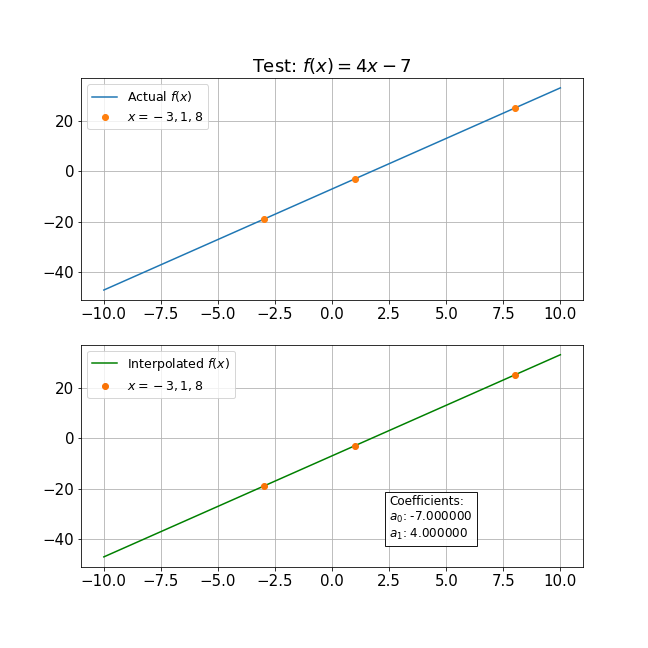
\includegraphics[scale = 0.4]{interp_test1}
 \caption{Plot and Interpolation of $f(x)=4x-7$}
 \label{fig:interp_test1}
\end{figure}

The first test was done with a simple linear equation (Figure \ref{fig:interp_test1}). Both the actual valued (top)
and the interpolated (bottom) functions are shown, with the corresponding calculated coefficients. With the success in
approximating the linear function, a more complicated cubic function was used for a second test, of which its
coefficients were also found, albeit with an almost zero coefficent for the $x^0$ term (Figure \ref{fig:interp_test2}).
\begin{figure}[h!]
 \centering
 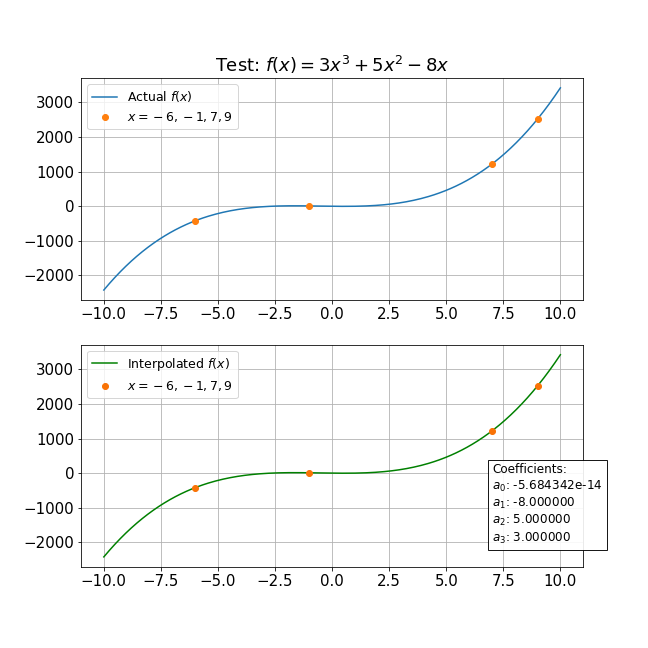
\includegraphics[scale = 0.4]{interp_test2}
 \caption{Plot and Interpolation of $f(x)=3x^3 + 5x^2 - 8x$}
 \label{fig:interp_test2}
\end{figure}
\vfill\eject
With the testing out of the way, the corresponding 5th degree polynomial for the given points was found and plotted from $x\in(-2.1, 2$), as
seen in Figure \ref{fig:interp}. The function evaluated at the desired points $x = -1, 0, 1$ can be seen in Table \ref{tab:interp_x}.
\begin{table}[h!]
 \centering
 \begin{tabular}{|c|c|}
 \hline
 \multicolumn{2}{|c|}{\textbf{Coefficients of $f(x)$}} \\
 \hline
 $a_0$ &  0.0725894\\
 $a_1$ & 1.70615614\\
 $a_2$ & 5.28873784\\
 $a_3$ & 1.33096305\\
 $a_4$ & -1.54167405\\
 $a_5$ & -0.5235626\\
 \hline
 \end{tabular}
 \caption{Coefficients of interpolated function}
 \label{tab:interp_coeff}
\end{table}
\begin{table}[h!]
 \centering
 \begin{tabular}{|c|c|c|}
 \hline
 $\boldsymbol{x}$ & $\boldsymbol{f(x)}$ & $\boldsymbol{\frac{d}{dx}f(x)}$ \\
 \hline
 $-1$ & $1.30609661$ & $-1.32954494$\\
 $0$ & $0.0725894$ & $1.70615747$\\
 $1$ & $6.33320977$ & $7.49200166$\\
 \hline
 \end{tabular}
 \caption{Evaluation of function and its derivative at select points}
 \label{tab:interp_x}
\end{table}
\vfill\eject
The first derivative of the function was then found using central finite differences and overplotted in order to
appreciate the location of their respective maxima and minima (Figure \ref{fig:interp}. The derivative evaluated at the points
$x=-1,0,1$ can also be seen in Table \ref{tab:interp_x}.
\begin{figure}[h!]
 \centering
 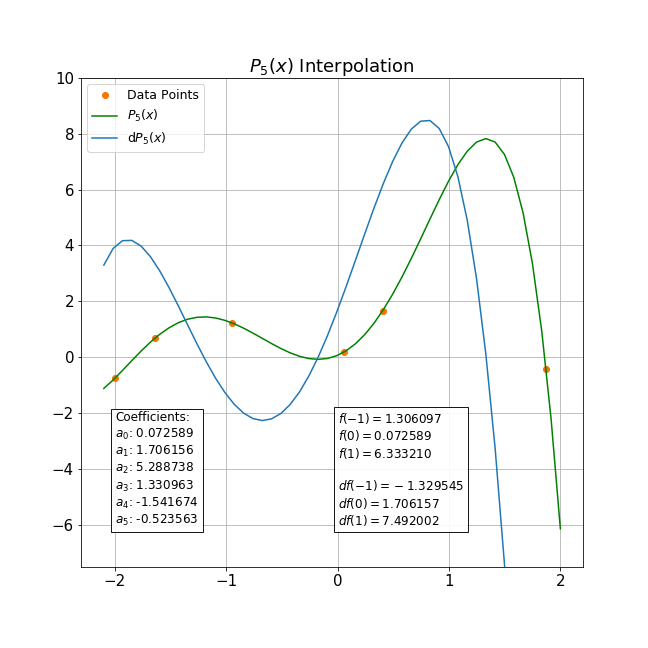
\includegraphics[scale = 0.4]{interp}
 \caption{Interpolated function and its derivative}
 \label{fig:interp}
\end{figure}

\section{Linear Algebra}

The algorithm for finding a solution to the system $\vec{x}$ to $A\vec{x} = \vec{b}$ was tested by analytically solving an arbitrary multplication between
a chosen matrix $A$ and a chosen vector $\vec{x}$. The resultant vector $\vec{b}$ when used as input for the algorithm along with the matrix $A$
should result with the same known $\vec{x}$. The used systems were:
\[\begin{bmatrix}
  1 & 2 \\
  3 & 4
 \end{bmatrix}
 \begin{bmatrix}
  5 \\
  7
 \end{bmatrix}
 =
 \begin{bmatrix}
  19 \\
  43
 \end{bmatrix}\]
\[\begin{bmatrix}
  2 & 1 & 1 \\
  1 & 2 & 1 \\
  1 & 1 & 2
 \end{bmatrix}
 \begin{bmatrix}
  1 \\
  2 \\
  3
 \end{bmatrix}
 =
 \begin{bmatrix}
  7 \\
  8 \\
  9
 \end{bmatrix}\]
With the algorithm being able to successfully find the appropriate $\vec{x}$ for each system.

The provided data for Problem 2 was imported and arranged as a 10x10 matrix, of which its upper left 2x2 submatrix is:
\[\begin{bmatrix}
 -0.69745 & -0.8223 \\
 -0.58764 & 0.14297
\end{bmatrix}\]

And its solution vector:
\[\vec{x} = 
 \begin{bmatrix}
  -0.12103834 \\
  1.3682304 \\ 
  0.19600827 \\ 
  0.7385038 \\ 
  -0.63966155 \\
  -1.28072921 \\ 
  0.11011213 \\ 
  0.69333823 \\ 
  0.71765722 \\
  0.38872449
 \end{bmatrix}\]

The the inverse matrix algorithm was tested by finding the inverse of the previously used example matrices (since they are simple enough to
determined by hand). After successfully obtaining the correct inverse matrices, the inverse for the given matrix A was able to be determined,
with its values at the indicated positions being shown in Table \ref{tab:inv}

\begin{table}[h!]
 \centering
 \begin{tabular}{|c|c|}
 \hline
 \textbf{Position} $\boldsymbol{A[i,j]}$ & \textbf{Value} $\boldsymbol{A_{ij}}$ \\
 \hline
 A[1,1] & -0.27238197 \\
 A[1,2] & 0.29591715 \\
 A[5,5] & -0.33018919 \\
 A[10,10] & -0.2538056 \\
 \hline
 \end{tabular}
 \caption{Values for the $A^{-1}$}
 \label{tab:inv}
\end{table}

\section{Root Finding:\\$f(x)=x^3 - x$}

The roots for this function can easily be determined analytically:
\begin{align*}
 0 &= x^3 - x \\
 0 &= x(x^2 - 1) \\
 x &= -1, 0, 1
\end{align*}

The roots are then approximated numerically using the Bisection and Newton-Raphson methods in Python, to an accuracy of $10^{-5}$.
\begin{figure}[h!]
 \centering
 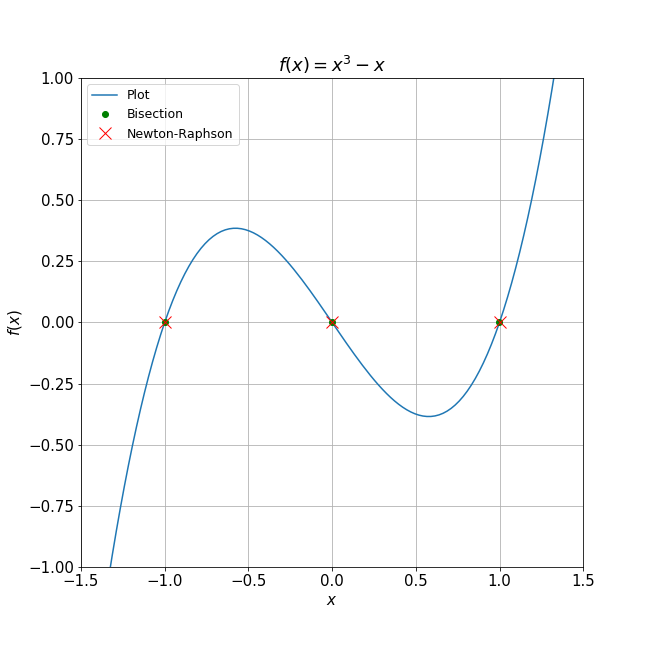
\includegraphics[scale = 0.4]{f3}
 \caption{Plot of function and calculated roots}
 \label{fig:f3}
\end{figure}

In order for the Bisection method to converge, a function's root must be preceded by negative values and proceded by positive values for said
function. If the root happens to be some sort of extrema, where ther is no change in sign for $f(x)$, then this method will fail.
In the case of this function, this rule is satisfied and so the roots can be approximated.

Newton-Raphson-s method on the other hand will converge as long as the derivative of the function is continuous in the interval $[a,b]$
where the root is believed to be and this interval does not enclose an extreme of the function.

The method was tested by attempting to find the root at decreasing interval sizes. It can be seen that
the root will be found regardless of size, as long as the interval used encloses it (Figure \ref{fig:f3_bitest}).
\begin{figure}[h!]
 \centering
 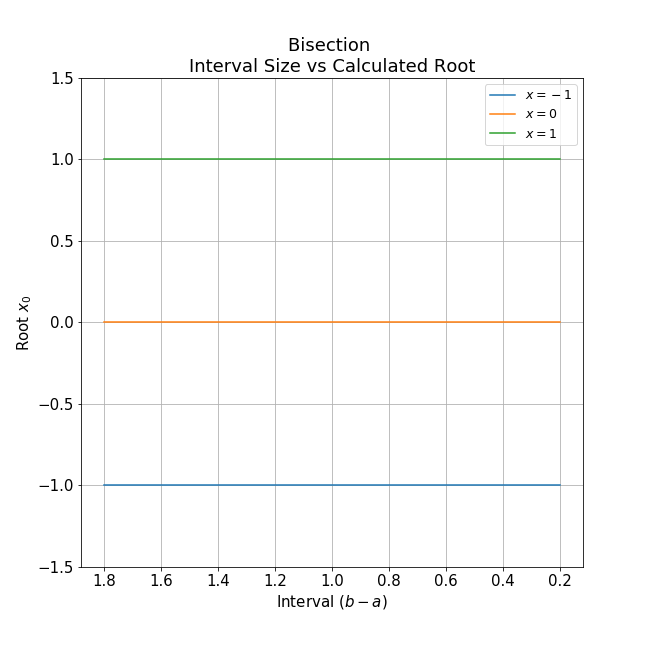
\includegraphics[scale = 0.4]{f3_bitest}
 \caption{Bisection: Plot of calculated root depending on interval size}
 \label{fig:f3_bitest}
\end{figure}

Newton-Raphson's method underwent the same test and it also converged to the root regardless of the interval size.
\begin{figure}[h!]
 \centering
 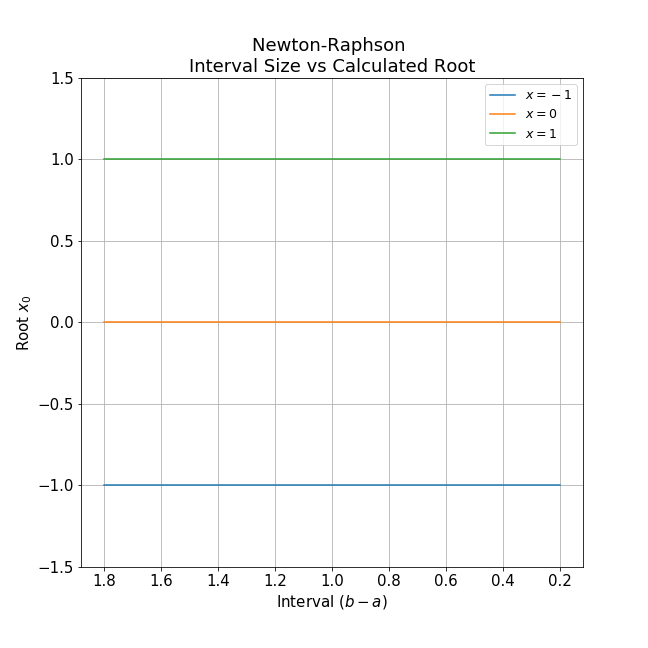
\includegraphics[scale = 0.4]{f3_nrtest}
 \caption{Newton-Raphson: Plot of calculated root depending on interval size}
 \label{fig:f3_nrtest}
\end{figure}

Care must be taken in both methods when choosing an interval, since they may not converge or skip roots if an interval is too large and contains
two or more roots.

\section{Root Finding:\\$f(x)=x^2-4xsinx+4sin^2x$}
This function can be simplified to:
\begin{equation*}
 f(x) = (x - 2sinx)^2
\end{equation*}

Which is still a tricky equation to solve analytically. To find the roots of the previous expression, WolframAlpha was used, as the engine is very dependable
and accurate handling mathematical operations.

The Bisection method was unable to find a root for this function due to its roots also being its local minima. Since there are no negative values for $f(x)$ before
or after the root, the Bisection method cannot function.

To find the root $x = 0$ with the Newton-Raphson method, it was necessary to have an interval where the values weren't mirrored ($|a|\neq |b|$). This
is due to the algorithm determining a point $x = (a + b)/2$ for a given interval $[a,b]$, which would result in the algorithim
dividing by $0$ ($df(0) = 0$!). So unlike the interval used in the previous problem ($[-0.6,0.6]$), the interval used to determine
the root $x=0$ was $(-0.5,0.6)$.

This function was also subject to the same test as in the previous problem, using decreasing interval sizes to see if there is a change in the evaluated root.

\begin{figure}[h!]
 \centering
 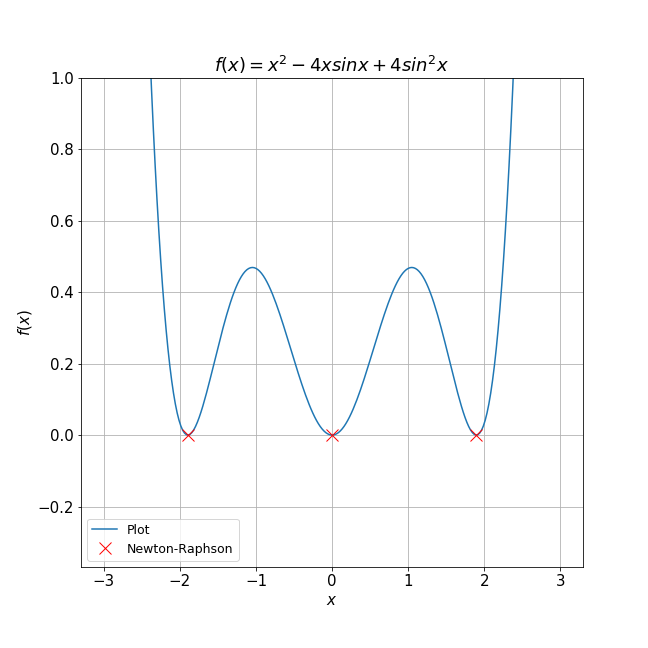
\includegraphics[scale = 0.4]{f4}
 \caption{Plot of function and calculated roots}
 \label{fig:f4}
\end{figure}

\vfill\eject
\section{Root Finding:\\Hermite Polynomials}
With the Bisection and Newton-Raphson methods thoroughly tested and proven functional, roots for the
Hermite polynomials $H_5$ and $H_6$ were approximated and compared to values obtained by Greenwood and Miller [1948].
Both methods were sucessfully able to find roots to both polynomials. Of the two methods, Newton-Raphson's calculated
roots were much closer to that of the used reference (Table \ref{}).
\begin{figure}[h!]
 \centering
 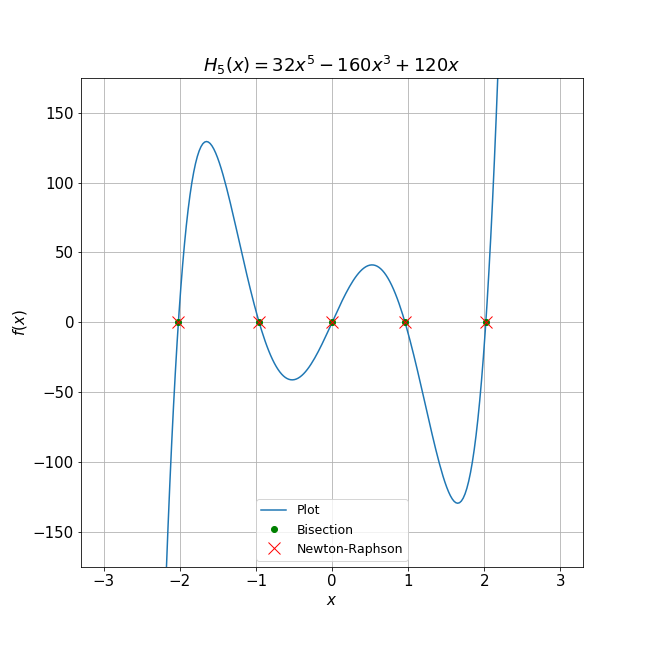
\includegraphics[scale = 0.4]{h5}
 \caption{Plot of $H_5$ and calculated roots}
 \label{fig:h5}
\end{figure}
\begin{figure}[h!]
 \centering
 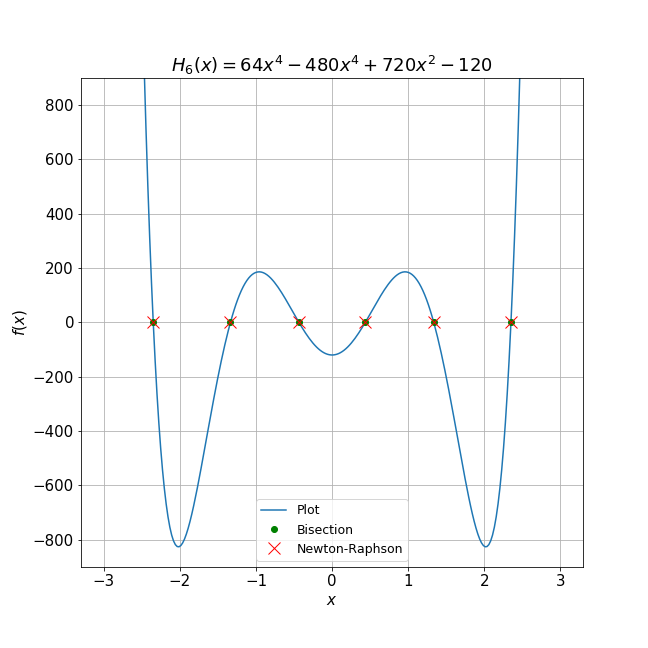
\includegraphics[scale = 0.4]{h6}
 \caption{Plot of $H_6$ and calculated roots}
 \label{fig:h6}
\end{figure}
\begin{table}[h!]
 \centering
 \begin{tabular}{|c|c|c|}
  \hline
  \multicolumn{3}{|c|}{Roots of Hermite Polynomials}\\
  \hline
  Greenwood \& Miller & Bisection & Newton-Raphson\\
  \hline
  \multicolumn{3}{|c|}{$\boldsymbol{H_5}$}\\
  \hline
  $0$ & $-4.5776367E-06$ & $-1.0148108e-10$\\
  $\pm0.9585725$ & $\pm-0.9585678$ & $\pm0.9585725$\\
  $\pm2.0201829$ & $\pm2.0201798$ & $\pm2.0201829$\\
  \hline
  \multicolumn{3}{|c|}{$\boldsymbol{H_6}$}\\
  \hline
  $\pm0.4360774$ & $\pm0.4360779$ & $\pm0.4360774$\\
  $\pm1.3558490$ & $\pm1.3358429$ & $\pm1.3358491$\\
  $\pm2.3506050$ & $\pm2.3506020$ & $\pm2.3506050$ \\
  \hline
 \end{tabular}
\caption{Value of roots to Hermite Polynomials $H_5$ and $H_6$}
\end{table}


\bibliographystyle{apalike}
\addcontentsline{toc}{section}{References}
\bibliography{HW02}
\nocite{*}

\end{document}
